\documentclass[math-font=newcm]{sjtuarticle}

% \usepackage[hybrid,citations,fencedCode,underscores=false]{markdown}

\usepackage[style=gb7714-2015]{biblatex}
\addbibresource{ref.bib}

\graphicspath{{figs/}}

\usepackage{float}

\def\dd{\mathrm{d}}

\usepackage{listings}
\captionsetup[lstlisting]{labelfont=bf,justification=justified}
\providecommand{\code}[2]{\lstinputlisting[language=#2,caption=\href{run:#1}{\ttfamily #1}]{#1}}
\providecommand{\codeRange}[4]{\lstinputlisting[language=#2,caption=\href{run:#1}{\ttfamily #1},firstline=#3,lastline=#4]{#1}}
\definecolor{grey}{rgb}{0.8,0.8,0.8}
\definecolor{darkgreen}{rgb}{0,0.3,0}
\definecolor{darkblue}{rgb}{0,0,0.3}
\lstset{%
    numbers=left, %行号
    numberstyle=\tiny\color{grey},
    showstringspaces=false,
    showspaces=false,%
    tabsize=4,%
    frame=shadowbox,%
    basicstyle={\ttfamily\small},%
    keywordstyle=\color{blue!80!black}\bfseries,%
    identifierstyle=,%
    commentstyle=\color{green!50!blue}\itshape,%
    stringstyle=\color{green!50!black},%
    rulesepcolor=\color{gray!20!white},
    breaklines,
    columns=flexible,
    extendedchars=false,
    mathescape=true,
    escapebegin=\color{green!50!blue}
}

\usepackage[linesnumbered,ruled]{algorithm2e}
\usepackage[colorlinks]{hyperref}

\title{作业2}
\author{LogCreative}
\begin{document}
\maketitle

\tableofcontents*
\clearpage

\section{第1题}

\subsection{问题}
Let
\begin{align*}
    \gamma(t)&=(t,t^2),\quad 0\leq t\leq 1,\\
    \eta(t)&=(2t+1,t^3+4t+1),\quad 0\leq t\leq 1,
\end{align*}
Note that $\gamma(1)$ and $\eta(0)$ intersect at $(1,1)$.
\begin{enumerate}
    \item Program to draw $\gamma(t)$ and $\eta(t)$.
    \item Do $\gamma(t)$ and $\eta(t)$ meet with $C^1$ continuity at the intersection?
    \item Do $\gamma(t)$ and $\eta(t)$ meet with $G^1$ continuity at the intersection?
\end{enumerate}

\subsection{绘图}

图 \ref{fig:p1} 展示了绘图结果,红色的线为 $\gamma(t)$,蓝色的线为 $\eta(t)$,它们相交于 $(1,1)$。

\begin{figure}[h]
    \centering
    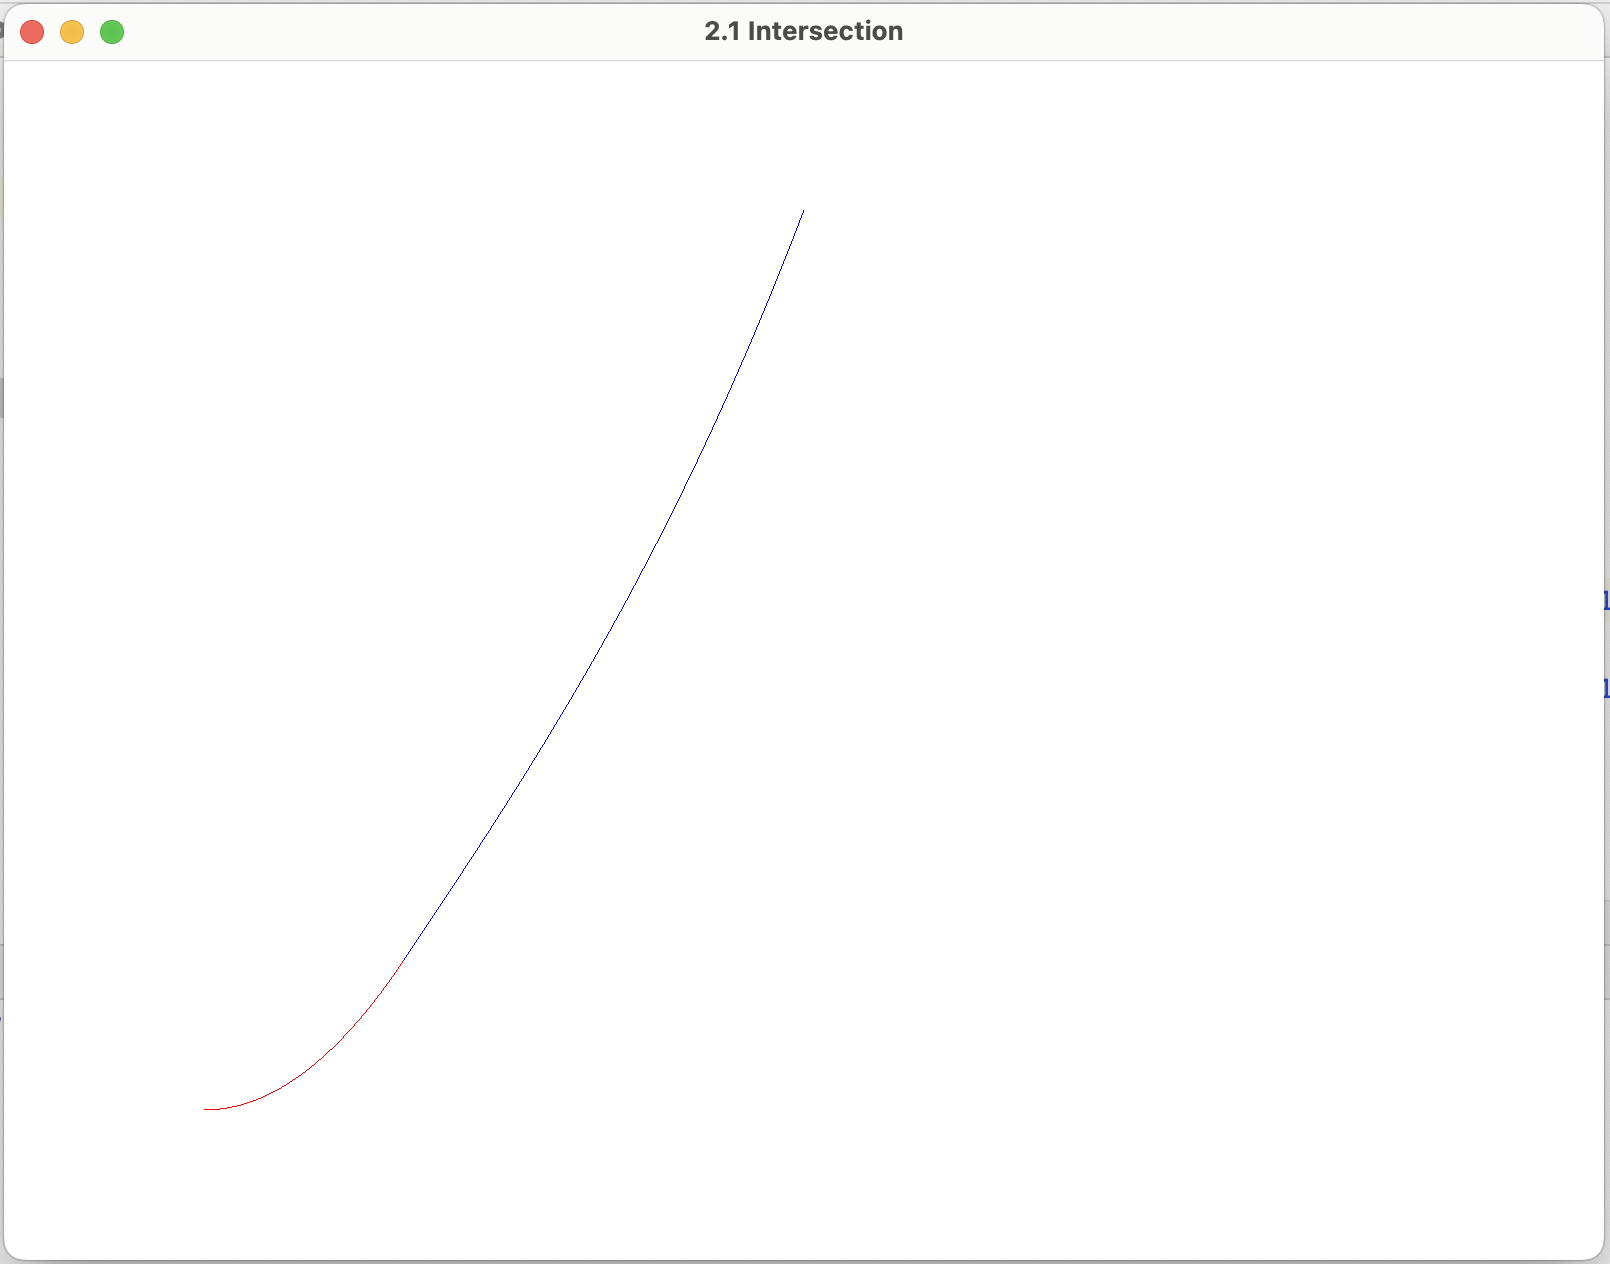
\includegraphics[width=0.8\textwidth]{p1.png}
    \caption{第1题绘图结果}
    \label{fig:p1}
\end{figure}

\subsection{连续性}

\textbf{它们在 $(1,1)$ 处不是 $C^1$ 连续的,但是是 $G^1$ 连续的。}

两者的切向量为

\begin{align}
    \frac{\dd}{\dd t}\gamma (t)&=\begin{pmatrix}\frac{\dd}{\dd t}t &\frac{\dd}{\dd t}t^2\end{pmatrix}^\top=\begin{pmatrix}1 & 2t \end{pmatrix}^\top \\
    \frac{\dd}{\dd t}\eta (t)&=\begin{pmatrix}\frac{\dd}{\dd t}(2t+1) &\frac{\dd}{\dd t}(t^3+4t+1)\end{pmatrix}^\top=\begin{pmatrix} 2 & 3t^2+4 \end{pmatrix}^\top
\end{align}

在 $(1,1)$ 处,有
\begin{align}
    \frac{\dd}{\dd t}\gamma (1)&=\begin{pmatrix}1 & 2 \end{pmatrix}^\top\\
    \frac{\dd}{\dd t}\eta (0)&=\begin{pmatrix} 2 & 4 \end{pmatrix}^\top
\end{align}

由于 $\begin{pmatrix}1 & 2 \end{pmatrix}^\top=\frac{1}{2}\begin{pmatrix} 2 & 4 \end{pmatrix}^\top$,所以它们方向相同,大小不同,在 $(1,1)$ 处不是 $C^1$ 连续的,方向相同导出它们是 $G^1$ 连续的。

\section{第 2 题}
\subsection{问题}
Let $t_0=0$, $t_1=1$, $t_2=3$, $t_3=4$, $t_4=5$. Using these values, compute $B_{0,4}$ and each of the functions used in its definition. Then plot these functions on the interval $-3\leq t\leq 8$.

\subsection{公式}

定义公式
\begin{align}
    B_{i,1}(t)&=\begin{cases}
        1, & t_i\leq t\leq t_{i+1},\\
        0, &\text{otherwise}
    \end{cases}\\
    B_{i,2}(t)&=\frac{t-t_i}{t_{i+1}-t_i}B_{i,1}(t)+\frac{t_{i+2}-t}{t_{i+2}-t_{i+1}}B_{i+1,1}(t)\\
    B_{i,3}(t)&=\frac{t-t_i}{t_{i+2}-t_i}B_{i,2}(t)+\frac{t_{i+3}-t}{t_{i+3}-t_{i+1}}B_{i+1,2}(t)\\
    B_{i,4}(t)&=\frac{t-t_i}{t_{i+3}-t_i}B_{i,3}(t)+\frac{t_{i+4}-t}{t_{i+4}-t_{i+1}}B_{i+1,3}(t)
\end{align}

可以导出

\begin{align*}
    &B_{0,1}(t)=\begin{cases}
        1, & 0\leq t\leq 1, \\
        0, & \text{otherwise}
    \end{cases} \quad B_{1,1}(t)=\begin{cases}
        1, & 1\leq t\leq 3, \\
        0, & \text{otherwise}
    \end{cases}\quad B_{2,1}(t)=\begin{cases}
        1, & 3\leq t\leq 4, \\
        0, & \text{otherwise}
    \end{cases}\quad B_{3,1}(t)=\begin{cases}
        1, & 4\leq t\leq 5, \\
        0, & \text{otherwise} 
    \end{cases}\\
    &B_{0,2}(t)=tB_{0,1}(t)+\frac{3-t}{2}B_{1,1}(t)\quad B_{1,2}(t)=\frac{t-1}{2}B_{1,1}(t)+\frac{4-t}{3}B_{2,1}(t) \quad B_{2,2}(t)=(t-3)B_{2,1}(t)+(5-t)B_{3,1}(t)\\
    &B_{0,3}(t)=\frac{1}{3}B_{0,2}(t)+\frac{4-t}{3}B_{1,2}(t)\quad B_{1,3}(t)=\frac{t-1}{3}B_{1,2}(t)+\frac{5-t}{2}B_{2,2}(t)\\
    &B_{0,4}(t)=\frac{t}{4}B_{0,3}(t)+\frac{5-t}{4}B_{1,3}(t)
\end{align*}

\subsection{绘图}

图 \ref{fig:p2} 展示了绘图结果,红色的线为 $B_{i,1}$(由浅到深、从左到右分别为 $i=0,1,2,3$);绿色的线为 $B_{i,2}$(由浅到深、从左到右分别为 $i=0,1,2$);蓝色的线为 $B_{i,3}$(由浅到深、从左到右分别为 $i=0,1$);黑色的线为最终结果 $B_{0,4}$。

\begin{figure}[h]
    \centering
    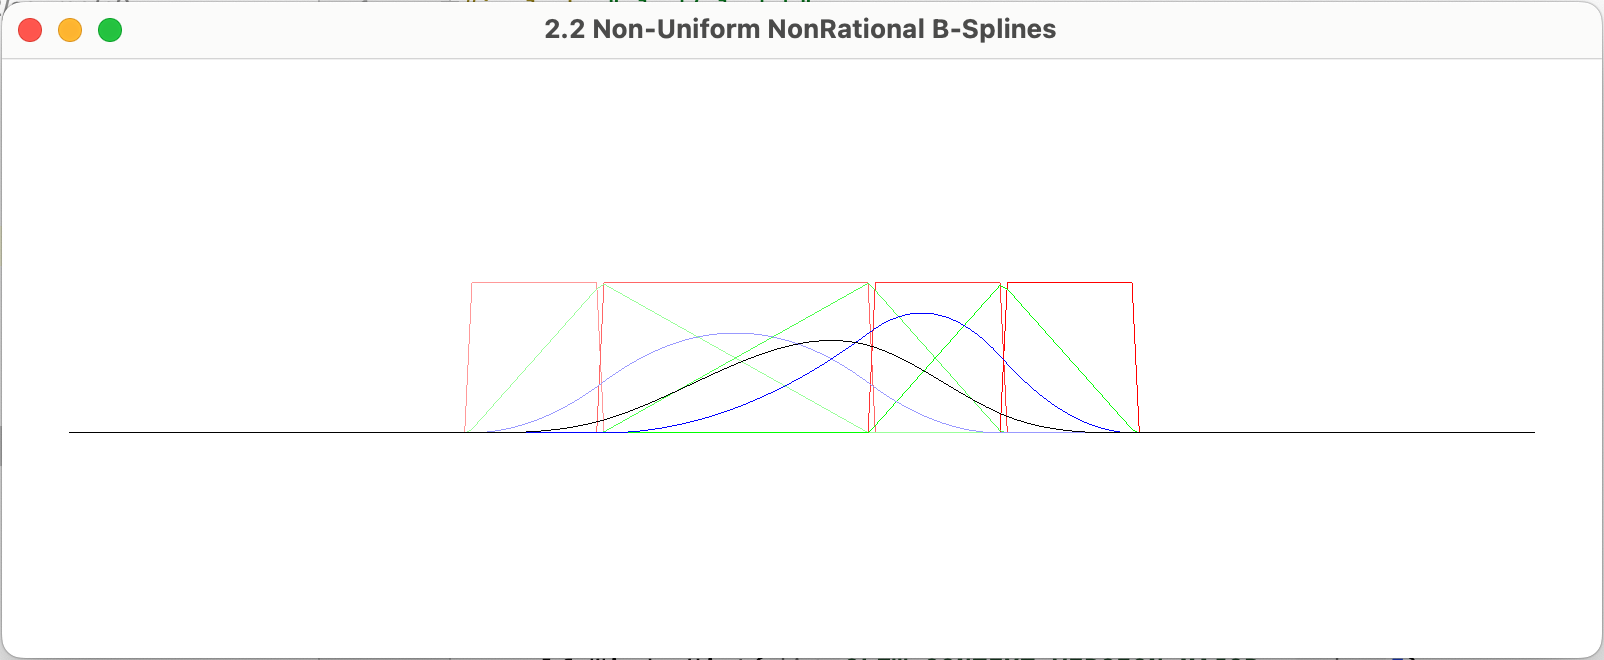
\includegraphics[width=0.8\textwidth]{p2.png}
    \caption{第2题绘图}
    \label{fig:p2}
\end{figure}

\appendix

\section{\texttt{FunctionDrawer} 类}

封装 \texttt{FunctionDrawer} 类定义绘制图像的操作。

\code{../source/p1/src/FunctionDrawer.h}{c++}

使用时先构造 \texttt{FunctionDrawer} 类来定义绘制的函数,然后 \texttt{init()} 初始化参数范围之内的坐标,在渲染过程中使用 \texttt{draw()} 绘制,最后结束程序时析构回收内存,比如下面的例子:

\codeRange{../source/p1/src/main.cpp}{c++}{43}{71}

\section{函数列表}

\subsection{第1题}

\code{../source/p1/src/MyFunctions.h}{c++}

\subsection{第2题}

\code{../source/p2/src/NUNRB.h}{c++}

\section{\texttt{Shader} 类的改动}

在 \parencite{shaders} 中 \texttt{Shader} 类的基础上增加了 \texttt{setVec4} 方法方便修改颜色。

\codeRange{../source/p1/src/shader\_s.h}{c++}{94}{97}

\section{编译方法}

分别打开 \verb"source/p1" 和 \verb"source/p2" 两个文件夹中的 CMake 工程进行编译。

\printbibliography[heading=bibintoc]


\end{document}